% !TEX program = xelatex

\documentclass[12pt,a4paper]{article}
\usepackage[UTF8]{ctex}
\usepackage{float}
\usepackage{amsmath}
\usepackage{amsfonts}
\usepackage{enumerate}
\usepackage{booktabs}
\usepackage{graphicx}
\usepackage{longtable}
\usepackage{subfigure}

\usepackage{url}
\usepackage{multirow}

% for plotting 
\usepackage{caption}
\usepackage{pgfplots}

% for pseudo code 
\usepackage{algorithm}
\usepackage[noend]{algpseudocode}

% for reference 
\usepackage{hyperref}
\usepackage{cleveref}

% for code 
\usepackage{listings}
\usepackage{xcolor}
\usepackage{fontspec}
\definecolor{darkgreen}{rgb}{0,0.6,0}
\newfontfamily\consolas{Consolas}

\usepackage{amssymb}
\usepackage{pifont}
\usepackage{xcolor}
\newcommand{\cmark}{\ding{51}}
\newcommand{\xmark}{\ding{55}}

\lstset {
    basicstyle=\footnotesize\consolas, % basic font setting
    breaklines=true, 
    frame=single,     % {single, shadowbox, bottomline}
    keywordstyle=\color{blue}, 
    commentstyle=\color{darkgreen},
    stringstyle=\color{red},
    showstringspaces=false,
    % backgroundcolor=\color{black!5}, % set backgroundcolor
    numbers=left, 
    numberstyle=\ttfamily,
}

% Microsoft Word A4 paper default layout 
\usepackage[a4paper, left=3.18cm, right=3.18cm, top=2.54cm, bottom=2.54cm]{geometry}

% \captionsetup[figure]{labelfont={bf}, name={Figure}}
% \captionsetup[table]{labelfont={bf}, name={Table}}

\crefname{equation}{方程}{方程}
\Crefname{equation}{方程}{方程}
\crefname{table}{表}{表}
\Crefname{table}{表}{表}
\crefname{figure}{图}{图}
\Crefname{figure}{图}{图}

\title{数学实验:第七次作业}
\author{计算机系 \quad 计73 \quad 2017011620 \quad 李家昊}
\date{\today}

% 实验报告格式的基本要求

% 系别、班级、学号、姓名

% 1 实验目的
% 2 题目
%   2.1 计算题:题号,算法设计(包括计算公式),程序,计算结果(计算机输出),结果分析,结论。
%   2.2 应用题:题号,问题分析,模型假设,模型建立,算法设计(包括计算公式),程序,计算结果(计算机输出),结果的数学分析,结果的实际意义,结论。
% 3 收获与建议

% Calc
% \subsubsection{算法设计}
% \subsubsection{程序}
% \subsubsection{计算结果}
% \subsubsection{结果分析}
% \subsubsection{结论}

% App
% \subsubsection{问题分析}
% \subsubsection{模型假设}
% \subsubsection{模型建立}
% \subsubsection{算法设计}
% \subsubsection{程序}
% \subsubsection{计算结果}
% \subsubsection{结果的数学分析}
% \subsubsection{结果的实际意义}
% \subsubsection{结论}

\begin{document}

\maketitle

\section{实验目的}

\begin{itemize}
    \item 练习建立实际问题的整数规划模型。
    \item 掌握用LINGO软件求解整数规划问题。
\end{itemize}

\section{问题求解}

\subsection{Chap10-Ex8 服务员聘用(应用题)}

% 8. 某储蓄所每天的营业时间是上午9 时到下午5 时。根据经验,每天不同时间段所需要的服务员数量如表10.7。
% 时间段(时) 9~10 10~11 11~12 12~1 1~2 2~3 3~4 4~5
% 服务员数量 4 3 4 6 5 6 8 8
% 储蓄所可以雇佣全时和半时两类服务员。全时服务员每天报酬100 元,从上午9 时到下午5 时工作,但中午12 时到下午2 时之间必须安排1 小时的午餐时间。储蓄所每天可以雇佣不超过3名的半时服务员,每个半时服务员必须连续工作4 小时,报酬40 元。问该储蓄所应如何雇佣全时和半时两类服务员。如果不能雇佣半时服务员,每天至少增加多少费用。如果雇佣半时服务员的数量没有限制,每天可以减少多少费用。

\subsubsection{问题分析}

题目给定储蓄所各时段的服务员数量要求,全时服务员和半时服务员的每日报酬和工作时间,需要确定聘用方案,这是一个整数规划问题。

\subsubsection{模型假设}

为了简化实际情况,模型基于以下假设,
\begin{enumerate}
    \item 总收益与服务员数量无关。
    \item 各时段的人流分布稳定,未来的人流分布与经验数据相差不大。
\end{enumerate}

\subsubsection{模型建立}

\paragraph{半时服务员不超过3名时} 在全时服务员中,设12时到1时午餐的人数为$x_1$,1时到2时午餐的人数为$x_2$,在半时服务员中,设9时到1时工作的人数为$y_1$,10时到2时工作的人数为$y_2$,11时到3时工作的人数为$y_3$,12时到4时工作的人数为$y_4$,1时到5时工作的人数为$y_5$,则各种服务员在各时段的工作时间表如\Cref{tab:ex8_task}所示。

\begin{table}[H]
    \centering
    \caption{各种服务员在各时段的工作时间表}
    \label{tab:ex8_task}
    \begin{tabular}{c|cccccccc}
        \toprule
        & $9\sim 10$ & $10\sim 11$ & $11\sim 12$ & $12\sim 1$ & $1\sim 2$ & $2\sim 3$ & $3\sim 4$ & $4\sim 5$\tabularnewline
        \midrule
        \(x_1\) & \cmark & \cmark &
        \cmark & & \cmark & \cmark
        & \cmark & \cmark\tabularnewline
        \(x_2\) & \cmark & \cmark &
        \cmark & \cmark & & \cmark
        & \cmark & \cmark\tabularnewline
        \(y_1\) & \cmark & \cmark &
        \cmark & \cmark & & & &\tabularnewline
        \(y_2\) & & \cmark & \cmark &
        \cmark & \cmark & & &\tabularnewline
        \(y_3\) & & & \cmark & \cmark &
        \cmark & \cmark & &\tabularnewline
        \(y_4\) & & & & \cmark & \cmark &
        \cmark & \cmark &\tabularnewline
        \(y_5\) & & & & & \cmark & \cmark &
        \cmark & \cmark\tabularnewline
        \bottomrule
    \end{tabular}
\end{table}

将工作时间表记为矩阵$\mathbf{A} \in \mathbb{R}^{7 \times 8}$,其中符号{\cmark}对应数值1,空白位置对应数值0。记各种服务员的聘用人数为$\mathbf{x} = (x_1, x_2, y_1, y_2, y_3, y_4, y_5)^T$,各时段服务员需求量为$\mathbf{b} = (4, 3, 4, 6, 5, 6, 8, 8)^T$,则需求量约束可表示如下,注意这里的$\ge$符号表示按分量比较,
\begin{equation}\label{eq:ex8_cons_demand}
    \mathbf{A}^T \mathbf{x} \ge \mathbf{b}
\end{equation}

半时服务员的最大数量约束为,
\begin{equation}\label{eq:ex8_cons_parttime}
    \sum_{i=1}^5 y_i \le 3
\end{equation}

还需要加上非负整数约束,
\begin{equation}\label{eq:ex8_cons_int}
    \mathbf{x} \in \mathbb{N}^7
\end{equation}

在此基础上,需要最小化每日人力成本$f$,
\begin{equation}\label{eq:ex8_obj}
    \min f = 100(x_1 + x_2) + 40(y_1 + y_2 + y_3 + y_4 + y_5)
\end{equation}

这就构成了一个整数规划模型,目标函数为\Cref{eq:ex8_obj},决策变量为$\mathbf{x}$,约束条件为\Cref{eq:ex8_cons_demand},\Cref{eq:ex8_cons_parttime}和\Cref{eq:ex8_cons_int}。

\paragraph{不能雇佣半时服务员时} 只需把半时服务员的约束条件\Cref{eq:ex8_cons_parttime}修改为,
\begin{equation}\label{eq:ex8_cons_no_parttime}
    y_i = 0, \quad i=1,2,3,4,5
\end{equation}

此时,目标函数为\Cref{eq:ex8_obj},决策变量为$\mathbf{x}$,约束条件为\Cref{eq:ex8_cons_demand},\Cref{eq:ex8_cons_no_parttime}和\Cref{eq:ex8_cons_int}。

\paragraph{半时服务员数量没有限制时} 只需把半时服务员的约束条件\Cref{eq:ex8_cons_parttime}去掉即可。此时,目标函数为\Cref{eq:ex8_obj},决策变量为$\mathbf{x}$,约束条件为\Cref{eq:ex8_cons_demand}和\Cref{eq:ex8_cons_int}。

\subsubsection{算法设计}

对于该整数规划模型,可采用LINGO求解,对应的LINGO模型类别为PILP (Pure Integer Linear Program),求解方法为分支定界法 (B-and-B)。

\subsubsection{程序}

请参见附录\ref{sec:ex8_code}。

\subsubsection{计算结果}

\paragraph{半时服务员不超过3名时} LINGO经过19次迭代,求得全局最优解,得到总人力成本$f$的最小值为820元,各决策变量的最优值为,
\begin{equation}
    x_1 = 3, \quad x_2 = 4, \quad y_1 = 0, \quad y_2 = 2, \quad y_3 = 0, \quad y_4 = 0, \quad y_5 = 1
\end{equation}

\paragraph{不能雇佣半时服务员时} LINGO经过0次迭代,求得全局最优解,得到总人力成本$f$的最小值为1100元,各决策变量的最优值为,
\begin{equation}
    x_1 = 5, \quad x_2 = 6, \quad y_1 = 0, \quad y_2 = 0, \quad y_3 = 0, \quad y_4 = 0, \quad y_5 = 0
\end{equation}

此时,相比于默认情况,每天需要增加的费用为280元。

\paragraph{半时服务员数量没有限制时} LINGO经过2次迭代,求得全局最优解,得到总人力成本$f$的最小值为560元,各决策变量的最优值为,
\begin{equation}
    x_1 = 0, \quad x_2 = 0, \quad y_1 = 6, \quad y_2 = 0, \quad y_3 = 0, \quad y_4 = 0, \quad y_5 = 8
\end{equation}

此时,相比于默认情况,每天可以减少的费用为260元。

\subsubsection{结果的数学分析}

从计算结果可以看出,可招聘的半时服务员的数量越多,总费用就越低,这是因为半时服务员的时薪比全时服务员更低,在合理的安排下,招聘越多半时服务员,越有利于降低总成本。

此外,在本题条件下,全局最优解不唯一,例如当半时服务员不超过3名时,以下也是一个全局最优解,每日最小费用同样为820元。
\begin{equation}
    x_1 = 3, \quad x_2 = 4, \quad y_1 = 0, \quad y_2 = 0, \quad y_3 = 2, \quad y_4 = 0, \quad y_5 = 1
\end{equation}

\subsubsection{结果的实际意义}

该计算结果具有一定的实际意义,可作为制定招聘方案的重要参考。在实际情况下,还需考虑节假日与工作日的服务员数量差异,服务人数及总收益与服务员数量的关系,以及人流分布的波动情况,根据实际情况对模型进行微调。

\subsubsection{结论}

半时服务员不超过3名时,储蓄所应当聘请7名全时服务员,其中3名在12时到1时午餐,另外4名在1时到2时午餐,还应当聘请3名半时服务员,其中2名在10时到2时工作,另外1名在1时到5时工作,此时每日总费用最低,为820元。

不能雇佣半时服务员时,储蓄所应当聘请11名全时服务员,其中5名在12时到1时午餐,另外6名在1时到2时午餐,此时每日总费用最低,为1100元。相比于默认情况,每天需要增加的费用为280元。

半时服务员数量没有限制时,储蓄所应当聘请14名半时服务员,其中6名在9时到1时工作,另外8名在1时到5时工作,此时每日总费用最低,为560元。相比于默认情况,每天可以减少的费用为260元。


\subsection{Chap10-Ex9 原油采购与加工(应用题)}

% 10. 轧钢有两道工序:粗轧和精轧。粗轧钢坯时由于各种随机因素的影响,得到的钢材的长度呈正态分布,其均值可由轧机调整,而方差是设备精度决定的,不能改变;精轧时将粗轧得到的钢材轧成规定的长度(可以认为没有误差)。如果粗轧后的钢材长度大于规定长度,精轧时要把多出的部分轧掉,造成浪费;如果粗轧后的钢材长度已经小于规定长度,则整根报废,浪费更大。问题是已知钢材规定的长度l 和粗轧后的钢材长度的均方差sigma,求可以调整的粗轧时钢材长度的均值m,使总的浪费最小。试从以下两种目标函数中选择一个,在l=2m,sigma=20cm 条件下求均值m:
% 1)每粗轧一根钢材的浪费最小;
% 2)每得到一根规定长度钢材的浪费最小。

\subsubsection{算法设计}

\paragraph{模型建立} 由题意,钢材的规定长度为$l$,粗轧得到的钢材长度服从正态分布$N(m,\sigma^2)$,记其概率密度函数为$f(x)$,累积分布函数为$F(x)$。

对于第1个目标函数,每粗轧一根钢材的浪费长度为,
\begin{equation}
    u(m) = \int_{-\infty}^l xf(x)dx + \int_l^{+\infty} (x-l)f(x)dx = m - l(1-F(l))
\end{equation}

对于第2个目标函数,每得到一根规定长度钢材的浪费长度为,
\begin{equation}
    v(m) = \frac{u(m)}{1-F(l)} = \frac{m}{1-F(l)} - l
\end{equation}

分别求出最佳均值$m$,使得$u(m)$和$v(m)$取最小值即可。

\paragraph{算法实现} 对于累积分布函数,可采用\texttt{normcdf}命令,对于最小值求解,可采用\texttt{fminunc}命令。

\subsubsection{程序}

请参见附录\ref{sec:ex9_code}。

\subsubsection{计算结果}

为了生产出合格的钢材并减少浪费,最佳均值$m$应当在2附近,首先画出区间[2,3]中的$u(m)$和$v(m)$图像,如\Cref{fig:ex9_waste}。可以看出,最小值在$m=2.3$附近,因此将其作为初值进行求解。

\begin{figure}[H]
    \centering
    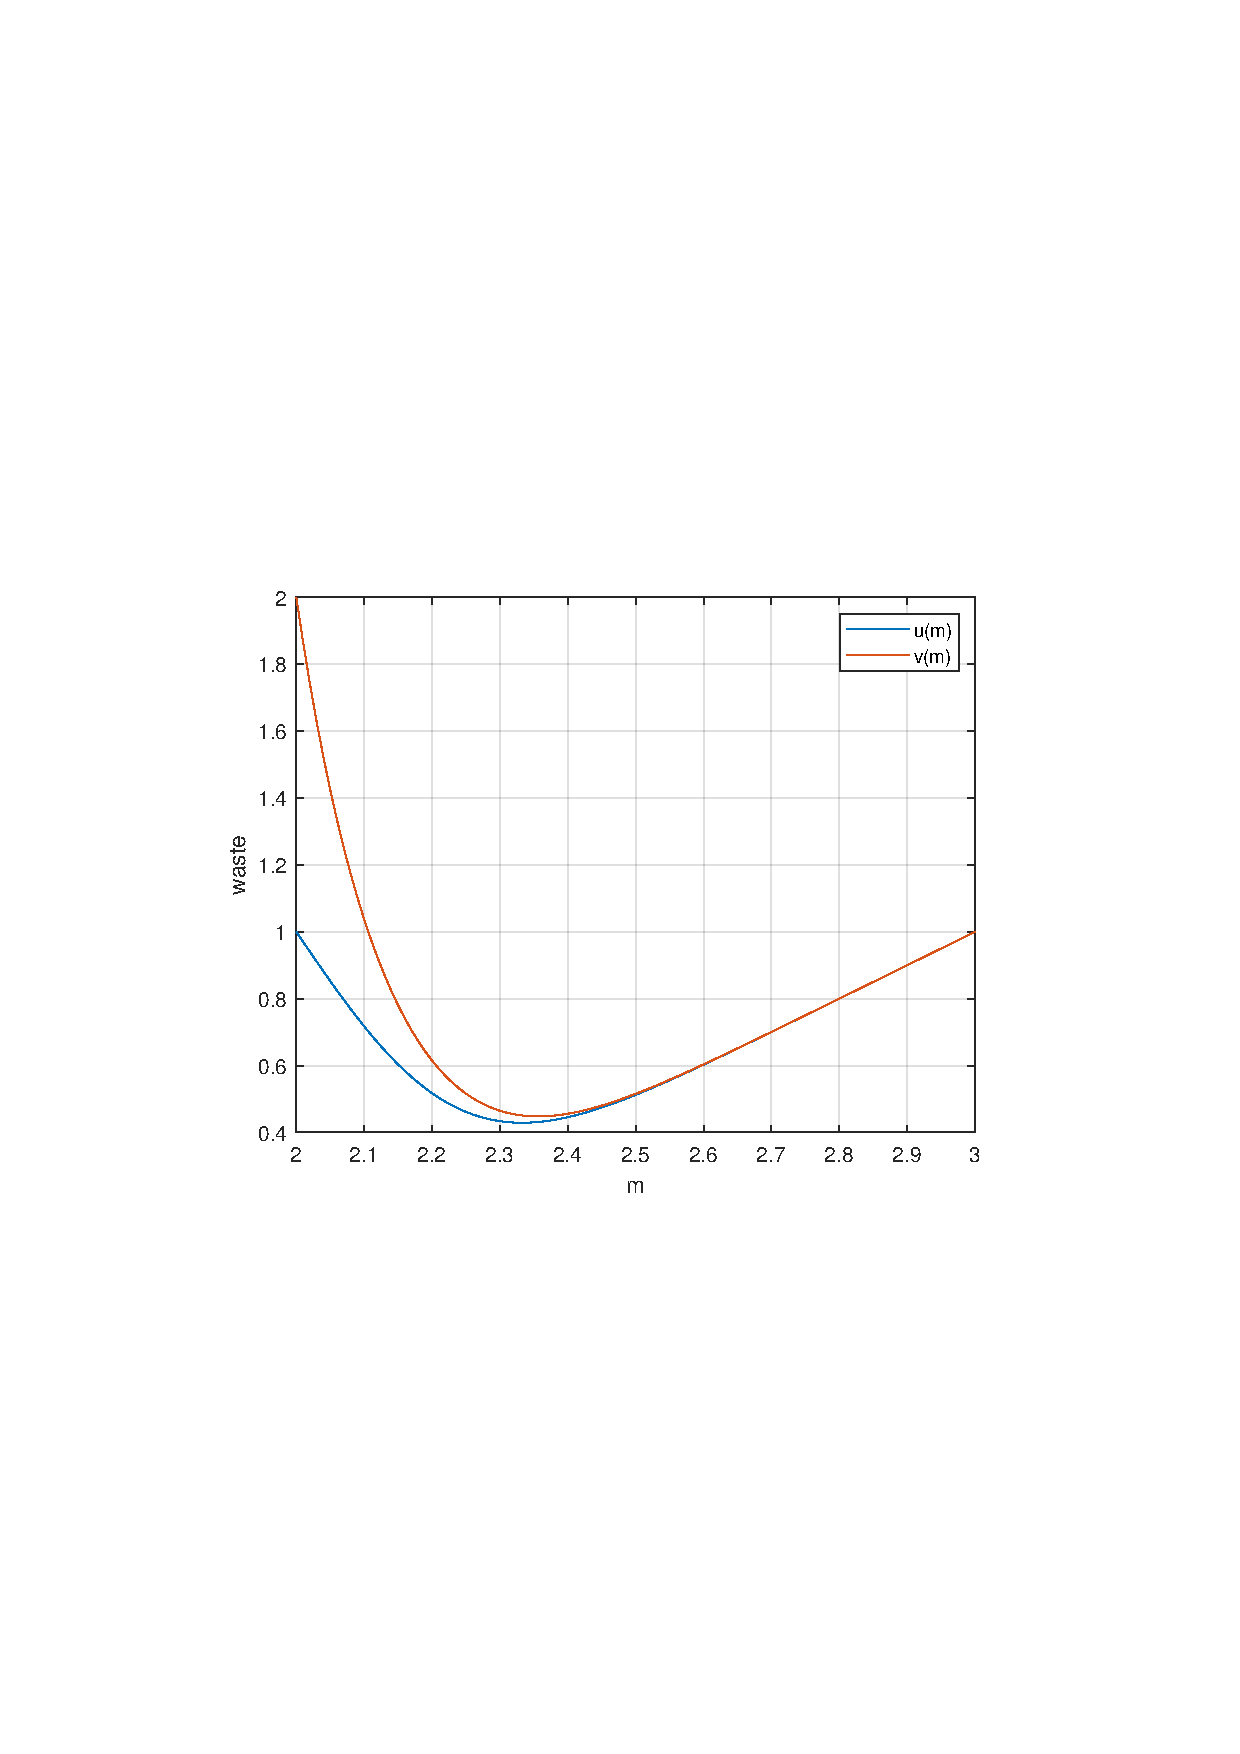
\includegraphics[width=0.8\textwidth,trim={3.09cm 9.295cm 3.09cm 9.295cm},clip]{fig/ex9_waste.pdf}
    \caption{两种目标函数的图像}
    \label{fig:ex9_waste}
\end{figure}

对于第1个目标函数,求解得到$m=2.3327$,此时浪费长度最小,为$u(m)=0.4289$。

对于第2个目标函数,求解得到$m=2.3562$,此时浪费长度最小,为$v(m)=0.4479$。

\subsubsection{结果分析}

由\Cref{fig:ex9_waste}可以看出,当$m$低于最优值时,粗轧得到钢管长度较短,导致整根报废的钢管数量较多,均摊到每根钢管的浪费长度较大;当$m$高于最优值时,粗轧得到的每根钢管长度较长,精轧时的浪费长度也较大;当$m$处于最优值时,达到了两者的平衡,此时平均浪费长度最小。

实际生产以利润为最终目标,生产利润往往与合格钢材的数量成正比,当生产每根合格钢材的浪费最小时,生产总利润最大,因此,在实际应用中,应当采用第2个目标函数。

\subsubsection{结论}

要求每粗轧一根钢材的浪费最小时,最优的粗轧钢材长度均值为2.3327米,此时平均浪费长度最小,为0.4289米。

要求每得到一根规定长度钢材的浪费最小时,最优的粗轧钢材长度均值为2.3562米,此时平均浪费长度最小,为0.4479米。


\subsection{Chap10-Ex11 钢管下料(应用题)}

% (钢管下料)某钢管零售商从钢管厂进货,将钢管按照顾客的要求切割后售出。从钢管厂进货时得到的原料钢管长度都是 1850 毫米。现有一客 户需要 15 根 290 毫米长、 28 根 315 毫米长、 21 根 350 毫米长和 30 根 455 毫米长的钢管。为了简化生产过程,规定所使用的切割模式的种类不能超过 4 种,使用频率最高的一种切割模式按照一根原料钢管价值的 1/10 增加费用,使用频率次之的切割模式按照一根原料钢管价值的 2/10 增加费用,依次类推,且每种切割模式下的切割次数不能太多(一根原料钢管最多生产 5 根产品)。此外,为了减少余料浪费,每种切割模式下的余料浪费不能超过 100 毫米。为了使总费用最小,应如何下料。

\subsubsection{问题分析}

题目设置了一个钢管生产场景,给出了原料钢管的长度,不同长度钢管的需求量,切割模式的成本,切割钢管的数量限制,需要确定最优生产方案,使得总费用最小。题目构成了一个钢管下料问题,这是一个经典的整数规划问题。

\subsubsection{模型假设}

为了简化实际情况,模型基于以下假设,
\begin{enumerate}
    \item 切割过程中没有物料损失,能够精准控制钢管长度,不产生次品。
    \item 生产余料的价值为零。
    \item 没有仓储和运输费用。
\end{enumerate}

\subsubsection{模型建立}

设用户需要$m$种规格的钢管,第$i$种规格的钢管长度为$d_i$,需求量为$c_i$,设一共采用$n$种切割模式,在第$j$种切割模式下,每根原料钢管的处理成本为$p_j$,共切割$x_j$根原料钢管,生产长度为$d_i$的钢管数量为$r_{ij}$,其中$i=1,2,\cdots,m$,$j=1,2,\cdots,n$。记原料钢管长度为$Q$,每种切割模式下余料的最大长度为$q$,每根原料钢管最多生产$k$根产品。

为方便叙述,记钢管长度向量$\mathbf{d} = (d_1,\cdots,d_m)$,需求向量$\mathbf{c} = (c_1,\cdots,c_m)$,生产矩阵$\mathbf{R} = (r_{ij})_{m \times n}$,原料消耗向量$\mathbf{x} = (x_1, \cdots, x_n)$,成本系数向量$\mathbf{p} = (p_1,\cdots,p_n)$。

为了使切割模式与价格对应,这里指定大小顺序为,
\begin{equation}\label{eq:ex11_cons_order}
    x_{j+1} \le x_j, \quad j=1,2,\cdots,n-1
\end{equation}

生产需要满足客户需求,注意这里的$\ge$符号表示按分量比较,
\begin{equation}\label{eq:ex11_cons_demand}
    \mathbf{Rx} \ge \mathbf{c}
\end{equation}

一根原料钢管最多生产$k$根产品,
\begin{equation}
    \sum_{i=1}^m r_{ij} \le k, \quad j=1,2,\cdots,n
\end{equation}

不同切割模式下需要满足余料限制,
\begin{equation}\label{eq:ex11_cons_remain}
    Q - q \le \mathbf{R}^T \mathbf{d} \le Q
\end{equation}

再加上非负整数约束,
\begin{equation}\label{eq:ex11_cons_int}
    \mathbf{x} \in \mathbb{N}^{m}, \quad \mathbf{R} \in \mathbb{N}^{m \times n}
\end{equation}

在此基础上,设每根原料钢管的采购成本为单位成本,需要最小化生产总费用$f$,
\begin{equation}\label{eq:ex11_objective}
    \min f = \mathbf{px}
\end{equation}

这是一个整数规划模型,目标函数为\Cref{eq:ex11_objective},决策变量为$\mathbf{R}$和$\mathbf{x}$,在约束条件\Cref{eq:ex11_cons_order},\Cref{eq:ex11_cons_demand},\Cref{eq:ex11_cons_remain}和\Cref{eq:ex11_cons_int}。

\subsubsection{算法设计}

对于整数规划,可以采用LINGO软件求解,需要使用\texttt{@gin}命令将决策变量限制在整数域内。

\subsubsection{程序}

请参见附录\ref{sec:ex11_code}。

\subsubsection{计算结果}

LINGO将该问题识别为PIQP (Pure Integer Quadratic Program),经过3,500,150次迭代,求得全局最优解,总费用$f$的最小值为21.5倍单位成本,决策变量$\mathbf{R}$和$\mathbf{x}$的最优值为,
\begin{equation}
    \mathbf{R} = \left(\begin{matrix}
        1 & 0 & 2 & 0\\
        2 & 0 & 0 & 0\\
        0 & 5 & 1 & 0\\
        2 & 0 & 2 & 4
    \end{matrix}\right)
    ,\quad
    \mathbf{x} = \left(\begin{matrix}
        14\\
        4\\
        1\\
        0
    \end{matrix}\right)
\end{equation}

将上述结果进行整理,得到具体切割模式及原料钢管消耗数量,如\Cref{tab:ex11_result}所示。注意到第四种切割模式的生产量为零,因此该切割模式无意义,应当将其省略。

\begin{table}[H]
    \centering
    \caption{具体切割模式及原料钢管消耗数量}
    \label{tab:ex11_result}
    \begin{tabular}{c|ccccc|c}
        \toprule
        & 290 mm & 315 mm & 350 mm & 455 mm & 余料 (mm) &
        原料钢管\tabularnewline
        \midrule
        切割模式1 & 1 & 2 & 0 & 2 & 20 & 14\tabularnewline
        切割模式2 & 0 & 0 & 5 & 0 & 100 & 4\tabularnewline
        切割模式3 & 2 & 0 & 1 & 2 & 10 & 1\tabularnewline
        \bottomrule
    \end{tabular}
\end{table}

\subsubsection{结果的数学分析}

整数规划是一个NPC问题,在求解过程中,往往需要通过增加约束条件,使得分支定界法能够及时剪枝,从而加快求解速度。额外的约束可以根据常理人为添加,也可以通过割平面算法求得。

在本题中,原料消耗量大小顺序约束\Cref{eq:ex11_cons_order}其实是不必要的,只要指定了成本系数向量$\mathbf{p}$,那么在最优解中,产量最大的切割模式必定对应最低的成本系数,否则,通过交换两种切割模式的顺序,就可以得到更低的成本。然而,如果将该约束去掉,则LINGO需要11,089,340次迭代才能求解出相同的结果,求解速度大约下降到了原来的1/4。

反过来,如果增加一个约束会怎么样呢?考虑到一根1850毫米长原料钢管的余料最多为100毫米,即使全部生产最长的455毫米长钢管,也至少生产4根才能满足余料约束,因此有,
\begin{equation}
    \sum_{i=1}^m r_{ij} \ge 4, \quad j=1,2,\cdots,n
\end{equation}

加上这个约束后,LINGO只需要828,566次迭代就能求出同样的结果,求解速度加快到了原来的4倍,因此附录的源码也增加了这个约束。

可见,在不改变最优解的情况下,约束越强,求解速度越快。

\subsubsection{结果的实际意义}

该计算结果具有一定的实用价值,可作为制定生产方案的重要参考。然而,该模型仍相对简单,在实际应用中,还应当综合考虑工厂的实际情况,例如原料钢管的运输费用,剩余成品的仓储成本,切割过程的物料损失,产品的次品率,余料的利用价值等因素,才能制定出合适的生产方案。

\subsubsection{结论}

应当使用三种切割模式。

第一种切割模式处理原料钢管14根,每根原料钢管切割成1根290毫米长,2根315毫米长和2根455毫米长钢管,余料为20毫米长。

第二种切割模式处理原料钢管4根,每根原料钢管切割成5根350毫米长钢管,余料为100毫米长。

第三种切割模式处理原料钢管1根,每根原料钢管切割成2根290毫米长,1根350毫米长和2根455毫米长钢管,余料为10毫米长。

此时总费用最小,为单根原料钢管采购成本的21.5倍。


\section{收获与建议}

在本次实验中,我掌握了LINGO软件求解整数规划的基本方法,用整数规划方法建立了实际问题的模型,并进行求解,在解决实际问题的过程中,我对数学方法的原理和应用有了更深刻的理解。

希望助教能对每次的实验进行详细的解答,希望老师在未来的课堂上介绍更多数学应用的前沿知识。

\section{附录:程序代码}

\subsection{Chap10-Ex8}\label{sec:ex8_code}

\lstinputlisting[language=Lingo]{../src/ex8.lng}

\subsection{Chap10-Ex9}\label{sec:ex9_code}

连续规划模型的代码如下,
\lstinputlisting[language=Lingo]{../src/ex9_cont.lng}

整数规划模型的代码如下,
\lstinputlisting[language=Lingo]{../src/ex9_int.lng}

\subsection{Chap10-Ex11}\label{sec:ex11_code}

\lstinputlisting[language=Lingo]{../src/ex11.lng}

\end{document}